\chapter{Presentasjon}
\begin{figure}[ht]
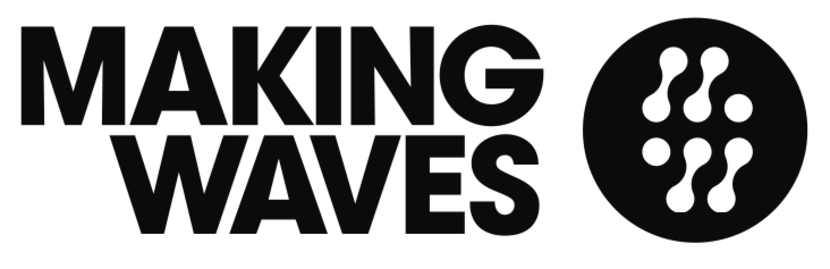
\includegraphics[scale=0.15, keepaspectratio]{./img/presentasjon/mw_logo.png}
\end{figure}
\begin{flushleft}
\renewcommand{\arraystretch}{1.5}
\begin{tabular}[ht]{@{}lp{100mm}@{}}
\textbf{Oppdragsgiver} & \href{http://www.makingwaves.no/}{Making Waves} 
(MW) \newline Kristian IVs gate 13 \newline 0164 Oslo \newline +47 22 206 020 \newline \href{mailto:post@makingwaves.com}{post@makingwaves.com} \\
\textbf{Prosjekteier} & \href{http://www.alpinanleggene.no/}{Alpinanleggenes Landsforbund} \\
\textbf{Prosjekttittel} & Fnugg \\ 
\textbf{Oppgave} & Utvidelser eller nyutvikling av en tjeneste tilknyttet løsningen \href{http://www.fnugg.no/}{Fnugg.no}. \\ 
\textbf{Periode} & 04.01.2016 - 28.05.2016 \\ 
\textbf{Gruppenummer} & 19 \\ 
\textbf{Gruppemedlemmer} & Espen Bjorøy Zaal - s198599 \newline Lukas David Larsed - s198569 \newline Henrik Fischer Bjelland - s198570\newline Simen Flatby - s198577 \\ 
\textbf{Gruppeleder} & Espen Bjorøy Zaal \\ 
\textbf{Intern veileder} & Thor E. Hasle \\ 
\textbf{Eksterne veiledere} & Marius Slette Johansen \newline Manager for Portals, Commerce and Data Analysis \newline \href{mailto:marius.johansen@makingwaves.no}{marius.johansen@makingwaves.no} \newline +47 982 48 333 \\
\textbf{Prosjektside} & \url{http://cerveceroscodigo.org/} \\
\end{tabular} 
\end{flushleft}

\section{Oppdragsgiver}
Making Waves er eksperter på digital tjenesteutvikling og innovasjon. Hos Making Waves finner du rådgivning, design, teknologi, innholdsproduksjon og drift under samme tak. Making Waves er en digital innovasjonspartner for mange av Nordens største merkevarer og offentlige virksomheter.

Making Waves ønsker å inkludere studentene i sine prosjekter gjennom å gi en oppgave som er løsbar på normert tid, og som vil utfordre og lære studentene til å bruke sin kunnskap og lære mer om utvikling, prosjekt og teknologi.

Oppgaven er tenkt å løse en utfordring i et prosjekt hvor det er muligheter for å gjøre utvidelser eller nyutvikling av en tjeneste tilknyttet løsningen Fnugg.no, en digital tjeneste for alpinanlegg og brukere av alpinanlegg. Løsningen eies av Alpinanleggenes Landsforbund.

Making Waves vil stille med faglig veiledning i prosjektet. Studentene kan forvente å jobbe sammen med Making Waves sine eksperter på .NET og søk.

\section{Oppgave}
Fnugg har et ønske om personalisering i fremtiden, og studentene vil få i oppgave å være med å se på konseptet personalisering gjennom utvikling av tjenester for innsamling av brukeradferd som skal lagres i CRM systemet, og tilgjengeliggjøring av data for videre personalisering gjennom API tjenester.

Det kan være aktuelt å benytte seg av Elastic Search som plattform for datainnsamling. Prosjektgruppen har skissert en arkitektur (se under) som er et godt utgangspunkt for videre definering av oppgaven i samsvar med hva prosjektet som helhet har som målsetning for 2016.

Oppgaven må avgrenses og vi ser det som urealistisk å inkludere betalingsløsning i oppgavens omfang.

Studentene forventes å sette seg inn i, og arbeide med, .NET, Elastic stacken (ELK), WEB API, Microsoft SQL, Microsoft Azure, Visual Studio.
